\documentclass[10pt]{beamer}

\usepackage[utf8]{inputenc}
\usepackage{tcolorbox}
\usepackage{tikz}
\usepackage{tikz-3dplot}
\usetikzlibrary{intersections,calc,,angles,quotes,through}
\usepackage{amsmath}
\usepackage{graphicx}
\usepackage{cases}
\def \heart {\textcolor{blue}{$\heartsuit$} }
\def \C {\mathcal{C}}
\def \orthog {\underline{\perp}}
\def\arcos{\operatorname{arcos}}

\tcbset{%
	basic/.style={colframe=black,
		      colback=white,
		      top= 0mm,
		      bottom = 2mm,
		      boxsep=0mm
		      }
}
\tikzset{
    invisible/.style={opacity=0},
    visible on/.style={alt={#1{}{invisible}}},
    alt/.code args={<#1>#2#3}{%
      \alt<#1>{\pgfkeysalso{#2}}{\pgfkeysalso{#3}} % \pgfkeysalso doesn't change the path
    },
  }

    
\begin{document}  
    \beamertemplatenavigationsymbolsempty
    \setlength{\abovedisplayskip}{0pt}
    \setlength{\belowdisplayskip}{0pt}
    \frame{
	  
	  \frametitle{Q1 Juillet 2002.}
	  \renewcommand{\theenumi}{\alph{enumi})}
	  Soit $ABC$ un triangle non rectangle, $\C$ son cercle circonscrit et $A'$ le point de $\C$
	  diamétralement opposé à $A$. La hauteur issue de $A$ coupe $A'B$ en $B'$, $A'C$ en $C'$
	  et $\C$ en $A$ et $E$.
	  \begin{enumerate}
	   \item Montrer que le triangle $A'B'C'$ est semblable au triangle $ABC$.
	   \item Prouver que les segments $[A',C]$ et $[B,E]$ ont même longueur.
	   \item Démontrer que le centre du cercle circonscrit au triangle $A'B'C'$ est sur la
		 tangente à $\C$ menée par $A'$.
	  \end{enumerate}

	  \vfill
	  
	  \pause
	  % hypothèses et thèse
	  \begin{tcolorbox}[basic] 
	      \begin{columns}[t]
		 
		 \column{.5\textwidth}\centering
		      
		      \underline{Hypothèses} 
		      \begin{itemize}
		      \item $AA'$ diamètre de $\C$,
		      \item $AE$ hauteur de $ABC$.
		      \end{itemize}

		  
		  \column{.5\textwidth}\centering
		      
		      \underline{Thèse} \\
		      \smallskip
		      \begin{enumerate}
		       \item $\Delta A'B'C',\Delta ABC$ semblables,
		       \item $|A'C| = |BE|$,
		       \item $O'A'\bot AA'$.		  
		      \end{enumerate}
		      {\small $O'$ centre du cercle circonscrit à $A'B'C'$.}
		
	      \end{columns}
	  \end{tcolorbox}
    }

    \frame{ 
	  % résolution ex1
	  \begin{columns}[t]
		\column{.548\textwidth}\centering 
		

			\underline{Dessin}\\
			
				  \begin{figure}[h]
				  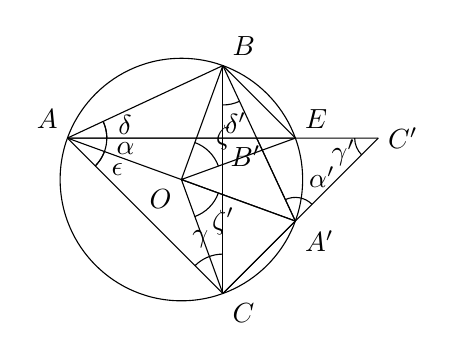
\begin{tikzpicture}[scale=0.77]
			          %projection ($(X)!(B')!(B)$)
			          %nommer chemin 'name path
			          %intersection \path [name intersections={of=d and gb,by=G}];
			          %animation  \draw[visible on=<1>] 
				  %           \draw[visible on=<{2,4}>]
				  %angle arc[radius = 6mm, start angle= 180, end angle= 225] node [below left,pos=0.3]{$\alpha$}
				  %angle \pic [draw, visible on=<2>, above left,"$\beta$", angle eccentricity=1.5] {angle = A'--A--B};
				  
				  %CERCLE et triangle
				  \coordinate (O) at (0,0);
				  \coordinate[label=above right:$B$] (B) at (70:2);
				  \coordinate[label=below right:$C$] (C) at (-70:2);
				  \coordinate[label=above left:$A$] (A) at (160:2);
				  \draw[name path =cercle] (O) circle (2);
				  \draw[] (A) -- (B);
				  \draw (C) -- (A);
				   \draw[visible on=<{1,2}>] (B) -- (C); 
				  
				  %A'
				  \coordinate[label=below right:$A'$] (A') at (-20:2);
				  \draw[] (A) -- (A');
				  %C'
				  \path[name path=A'C] (C) -- +($3*(A')-3*(C)$);
				  \path[name path =AC'] (A)--+(6,0);
				  \path[name intersections={of=A'C and AC',by=C'}];
				  \draw[visible on=<{1,2}>] (C) -- (C') node[right]{$C'$};
				  \draw[visible on=<{3}>] (A') -- (C);
				  \draw[visible on=<{1,2}>] (A) -- (C'); 
				  
				  %B'$
				  \draw [visible on=<{1,2}>,name path=A'B] (A') -- (B);
				  \path [name intersections={of=A'B and AC',by=B'}];			  
				  \draw [visible on=<{1,2}>] (A') -- (B') node[label=below left:$B'$,xshift=3mm,yshift=1.5mm]{};
				  %E%
				  \path [name intersections={of=cercle and AC',by=E}];
				  
				  \draw[visible on=<{2,3}>] (B) -- (E) node[above right]{$E$};
				  \draw[visible on=<{3}>] (A) -- (E);				  
				  %OB,OE,OA',OC
				  \draw[visible on=<3>] (O) node[below left]{$O$} -- (B) (O) -- (E) (O)--(A') (O) -- (C);
				  %angles 
				  \pic [draw, visible on=<1>,"$\alpha$", angle eccentricity=1.5] {angle = C--A--B};
				  \pic [draw, visible on=<1>,"$\alpha'$",above right, angle eccentricity=1,angle radius=3mm] {angle = C'--A'--B'};
				  \pic [draw, visible on=<1>,"$\gamma$", angle eccentricity=1.5] {angle = B--C--A};
				  \pic [draw, visible on=<1>,"$\gamma '$", angle eccentricity=1.6,angle radius=3mm] {angle = B'--C'--A'};
				  
				  \pic [draw, visible on=<{2,3}>,"$\delta$", angle eccentricity=1.5] {angle = B'--A--B};
				  \pic [draw, visible on=<{2,3}>,"$\epsilon$", angle eccentricity=1.5] {angle = C--A--A'};
				  \pic [draw, visible on=<2>,"$\delta '$", angle eccentricity=1.5] {angle = C--B--A'};
				  \pic [draw, visible on=<3>,"$\zeta$", angle eccentricity=1.5] {angle = E--O--B};
				  \pic [draw, visible on=<3>,"$\zeta '$", angle eccentricity=1.5] {angle = C--O--A'};
				  \end{tikzpicture}
				  \end{figure}
			
				  \begin{tcolorbox}[basic] 
				      
				    \smallskip
				    \underline{Hypothèses} 
				    \begin{enumerate}
				    \item $AA'$ diamètre de $\C$,
				    \item $AE$ hauteur de $ABC$.
				    \end{enumerate}
							      
				    \underline{Thèse} 
				    \renewcommand{\theenumi}{\alph{enumi})}
				    \begin{enumerate}
				    \item $\Delta A'B'C',\Delta ABC$ semblables,
				    \item $|A'C| = |BE|$,
				    \item $O'A'\bot AA'$.	
				    \end{enumerate}
				    \end{tcolorbox}
		
		
		\column{.54\textwidth}\centering
		
		\underline{Résolution}\\ \flushleft
		\onslide<+->\heart 2 $\Delta$ sont semblables si 2 angles de l'un sont égaux à deux angles de l'autre.
		\begin{enumerate}
		 \item $\alpha = \alpha '$, 
		 \item $\beta = \beta '$. (angles à côtés $\bot$)
		\end{enumerate}
		$\Delta A'B'C',\Delta ABC$ semblables.  \hfill $\qed(a)$
		\centering\noindent\rule{2cm}{0.4pt}\flushleft
			     \begin{align*}
	                      \onslide<+->{\delta =& \delta ', \text{ (angles à côtés $\bot$)} \\
					  \delta =& \epsilon, \text{ (angles inscrits)} \\}
			      \onslide<+->{2\zeta=& 2\zeta ', \\
					    \zeta=& \zeta ' \text{ $\rightarrow \Delta OBE,\Delta OCA'$ isométriques. } \\[1em]
					    &|A'C| = |BE|. \\
					    &\omit\hfill \qed(b)\\}	      
	                     \end{align*}
		

   
	   \end{columns}
    
    
    
    }
	  
	  \frame{ 
	  % résolution ex1
	  \begin{columns}[t]
		\column{.548\textwidth}\centering 
		

			\underline{Dessin}\\
				  \vspace{-6mm}
				  \begin{figure}[h]
				  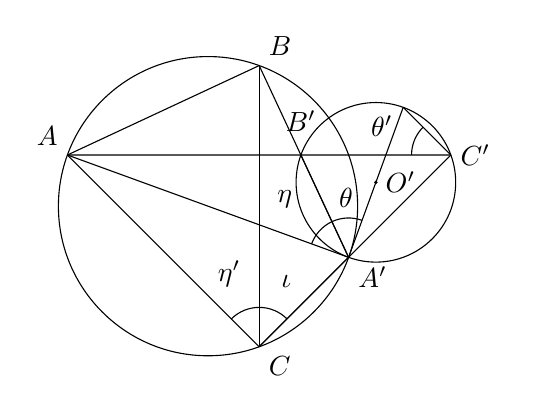
\begin{tikzpicture}[scale=0.95]
			          %projection ($(X)!(B')!(B)$)
			          %nommer chemin 'name path
			          %intersection \path [name intersections={of=d and gb,by=G}];
			          %animation  \draw[visible on=<1>] 
				  %           \draw[visible on=<{2,4}>]
				  %angle arc[radius = 6mm, start angle= 180, end angle= 225] node [below left,pos=0.3]{$\alpha$}
				  %angle \pic [draw, visible on=<2>, above left,"$\beta$", angle eccentricity=1.5] {angle = A'--A--B};
				  
				  %CERCLE et triangle
				  \coordinate (O) at (0,0);
				  \coordinate[label=above right:$B$] (B) at (70:2);
				  \coordinate[label=below right:$C$] (C) at (-70:2);
				  \coordinate[label=above left:$A$] (A) at (160:2);
				  \draw[name path =cercle] (O) circle (2);
				  \draw (A) -- (B);
				  \draw (C) -- (A);
				   \draw (B) -- (C); 
				  
				  %A'
				  \coordinate[label=below right:$A'$] (A') at (-20:2);
				  \draw (A) -- (A');
				  %C'
				  \path[name path=A'C] (C) -- +($3*(A')-3*(C)$);
				  \path[name path =AC'] (A)--+(6,0);
				  \path[name intersections={of=A'C and AC',by=C'}];
				  \draw (C) -- (C') node[right]{$C'$};
				  \draw (A') -- (C);
				  \draw (A) -- (C'); 
				  
				  %B'$
				  \draw [name path=A'B] (A') -- (B);
				  \path [name intersections={of=A'B and AC',by=B'}];			  
				  \draw (A') -- (B') node[label=above :$B'$,xshift=0,yshift=0.5mm]{};
				  				 
				  %Tangente
				  \path[name path=tangente] (A') -- ($(A')!3cm!-90:(A)$);
				  
				  %O'
				  \coordinate[] (M) at ($(A')!0.5!(C')$);
				  \path[name path =MO'] (M) -- ($(M)!2cm!90:(C')$);
				  \path [name intersections={of=MO' and tangente,by=O'}];
				  \coordinate[label=right:$O'$] () at (O');
				  \fill (O') circle (0.025);
				  
				  %C'
				  \node [draw, name path=cercle'] at (O') [circle through=(A')] {};
				  
				  \path [name intersections={of=cercle' and tangente,by=inter}];
				  \draw (A') -- (inter);
				  \draw (C') -- (inter);
				
				  %angles 
				  \pic [draw,"$\eta$", angle eccentricity=2.2] {angle = B--A'--A};
				  \pic [draw,"$\eta '$", angle eccentricity=2] {angle = B--C--A};
				  \pic [draw,"$\theta$", angle eccentricity=1.5] {angle = O'--A'--B'};
				  \pic [draw,"$\theta '$", angle eccentricity=1.9] {angle = inter--C'--B'};
				  \pic [draw,"$\iota$", angle eccentricity=1.8] {angle = A'--C--B};
				  \end{tikzpicture}
				  \end{figure}
				  \vspace{-4.5mm}
				  \begin{tcolorbox}[basic] 
				      
				    \smallskip
				    \underline{Hypothèses} 
				    \begin{enumerate}
				    \item $AA'$ diamètre de $\C$,
				    \item $AE$ hauteur de $ABC$.
				    \end{enumerate}
							      
				    \underline{Thèse} 
				    \renewcommand{\theenumi}{\alph{enumi})}
				    \begin{enumerate}
				    \item $\Delta A'B'C',\Delta ABC$ semblables,
				    \item $|A'C| = |BE|$,
				    \item $O'A'\bot AA'$.	
				    \end{enumerate}
				    \end{tcolorbox}
		
		
		\column{.54\textwidth}\centering
		
		\underline{Résolution}\\ \flushleft
		\begin{align*}
		 \widehat{AA'O'}=& \eta + \theta , \\
				=& \eta'+ \theta', \text{ (angles inscrits)} \\
				=& \eta'+ \iota', \text{ (angles à cotés $\bot$)} \\
				=& 90^{\circ}.			        
		\end{align*} 
		
		\bigskip
		
		$O'$ appartient à la tangente en $A'$. \hfill $\qed$
		

   
	   \end{columns}
    
            }
  
\end{document}
